\documentclass{beamer}

\usecolortheme[light]{solarized}

\beamertemplatenavigationsymbolsempty


\usepackage{graphicx}
\usepackage{hyperref}
\usepackage{tikz}
\usetikzlibrary{calc, patterns}



\begin{document}

    \begin{frame}
        \begin{center}
            \Large
            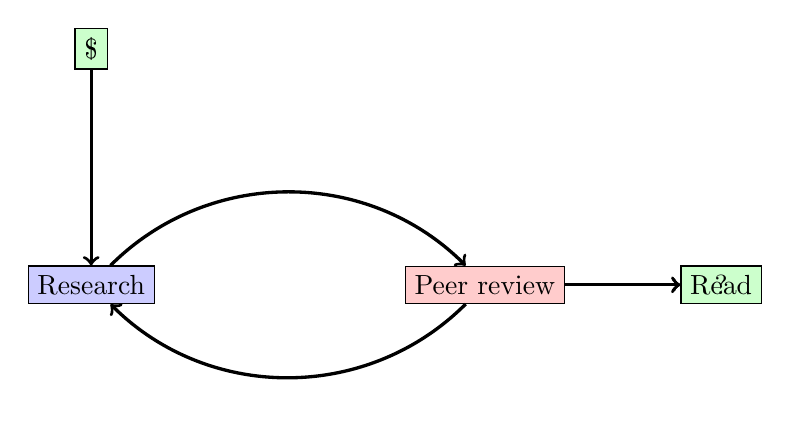
\begin{tikzpicture}
                \onslide<1-5, 6>{
                    \node (rsc) [draw, fill=blue!20] at (0, 0) {Research};
                    \node (peerreview) [draw, fill=red!20] at ($(rsc) + (5, 0)$) {Peer review};
                    \draw [->, very thick] (rsc) edge [out=45, in=135] (peerreview);
                    \draw [->, very thick] (peerreview) edge [in=-45, out=-135] (rsc);
                }
                \onslide<2-4>{
                    \node (read) [draw, fill=green!20] at ($(peerreview) + (3, 0)$) {Read};
                }
                \onslide<2-3>{
                    \draw [->, very thick] (peerreview) -- (read);
                }
                \onslide<3-5>{
                    \node (money) [draw, fill=green!20] at ($(rsc) + (0, 3)$) {\$};
                    \draw [->, very thick] (money) -- (rsc);
                }
                \onslide<4>{
                    \draw [->, dashed, thick] (peerreview) -- (read);
                }
                \onslide<5>{
                    \draw [->, dashed, thick] (peerreview) -- (read) node {?};
                }
            \end{tikzpicture}
        \end{center}
    \end{frame}

    \begin{frame}
        \begin{center}
            \onslide<2>{\Huge``}
            \Large
            \onslide<1, 2>{
                The work is unclear and I do not like it.
            }
            \onslide<2>{\Huge''}
        \end{center}
    \end{frame}

    \begin{frame}
        \Huge
        \begin{center}
            \url{http://joss.theoj.org/}
        \end{center}
    \end{frame}

\end{document}
